\subsubsection{2.2. Tiền xử lý dữ liệu}
\indent\indent Quy trình tiền xử lý dữ liệu đóng vai trò then chốt trong việc chuẩn hóa đầu vào cho mô hình đa phương thức. Quy trình này được thực hiện tuần tự qua 5 bước chính như sau:\vspace{-0.1cm}
\begin{itemize}[label={--}, itemsep=1pt]
    \item \textbf{Bước 1 -- Phân đoạn video và phụ đề:} Chia tách video gốc thành các mẫu dữ liệu (video clip) có độ dài cố định, đồng thời trích xuất phụ đề tương ứng.
    \item \textbf{Bước 2 -- Trích xuất hình ảnh và âm thanh:} Tách video clip thành chuỗi hình ảnh (frames) và các đoạn âm thanh (audio segments) theo tần số lấy mẫu quy định.
    \item \textbf{Bước 3 -- Chuẩn hóa phụ đề:} Sử dụng các mô hình ngôn ngữ lớn (LLM) để hiệu chỉnh và làm sạch dữ liệu phụ đề.
    \item \textbf{Bước 4 -- Tiền tính toán:} Trích xuất trước các đặc trưng văn bản và âm thanh, chuyển đổi sang định dạng vector/ma trận lưu trữ sẵn nhằm giảm tải chi phí tính toán trong quá trình huấn luyện.
    \item \textbf{Bước 5 -- Phân chia tập dữ liệu:} Chia tách dữ liệu thành các tập Train, Val và Test.
\end{itemize}
%============================================================================
\paragraph{2.2.1. Phân đoạn video và phụ đề}
\indent\indent Từ nguồn dữ liệu thô ban đầu, thư viện \textit{ffmpeg} được sử dụng để phân đoạn các video gốc thành các video clip nhỏ, mỗi clip có thời lượng chuẩn là 1 phút. Đây được coi là một mẫu dữ liệu (sample) đầu vào.\vspace{0.3cm}

Đối với việc xử lý phụ đề (định dạng \texttt{.srt} tải từ thư viện \textit{yt-dlp}), thách thức lớn nhất là sự không đồng bộ giữa mốc thời gian của phụ đề và thời điểm cắt video. Để khắc phục vấn đề này, quá trình cắt không được thực hiện theo cách ràng buộc cứng nhắc theo timestamp, mà thay vào đó áp dụng cơ chế cửa sổ chồng lấn (overlapping window). Nếu thời điểm bắt đầu hoặc kết thúc của một dòng phụ đề nằm trong khoảng thời gian của video clip, toàn bộ nội dung dòng phụ đề sẽ được giữ lại. Điều này đảm bảo ngữ nghĩa của câu nói không bị ngắt quãng, dù chấp nhận việc phụ đề có thể lấn sang khung thời gian trước hoặc sau video một khoảng nhất định.\vspace{0.3cm}

Sau quá trình cắt, bước lọc thủ công được tiến hành tiếp tục nhằm nâng cao chất lượng dữ liệu. Các video clip có thời lượng ngắn hơn 1 phút hoặc chứa nội dung nhiễu, không phù hợp với chủ đề của tập dữ liệu, sẽ bị loại bỏ trước khi đưa vào các giai đoạn xử lý và phân tích tiếp theo.\vspace{0.3cm}
%============================================================================
\paragraph{2.2.2. Trích xuất hình ảnh và âm thanh}
\indent\indent Tại bước này, mỗi mẫu dữ liệu (video clip 1 phút) sẽ được tách thành hai thành phần phương thức riêng biệt sử dụng \textit{ffmpeg}:\vspace{-0.1cm}
\begin{itemize}[label={--}, itemsep=1pt]
    \item Đối với hình ảnh: Thực hiện lấy mẫu (sampling) với chu kỳ 4 giây/khung hình. Như vậy, mỗi mẫu dữ liệu sẽ cung cấp một danh sách gồm 15 hình ảnh.
    \item Đối với âm thanh: Cũng thực hiện lấy mẫu với chu kỳ 5 giây/đoạn. Tương ứng mỗi mẫu dữ liệu sẽ cung cấp 12 đoạn âm thanh.
\end{itemize}
%============================================================================
\paragraph{2.2.3. Chuẩn hóa phụ đề}
\indent\indent Các đoạn phụ đề sau khi cắt sẽ được chuyển đổi sang định dạng văn bản thuần (\texttt{.txt}). Do đặc thù là văn bản nói và được tạo tự động, dữ liệu này thường chứa lỗi ngữ pháp, từ ngữ địa phương hoặc sai sót do nhận dạng âm thanh.\vspace{0.3cm}

Để nâng cao chất lượng dữ liệu văn bản, đề tài đề xuất sử dụng các LLM như GPT-5.0, GPT-4o hoặc Gemini 2.5 Pro để thực hiện tác vụ làm mượt. Các mô hình này hỗ trợ hiệu chỉnh ngữ pháp, tái cấu trúc câu từ cho mạch lạc mà vẫn giữ nguyên ý nghĩa gốc. Sau đó, cần phải tiến hành rà soát thủ công lần cuối để loại bỏ các mẫu không đạt yêu cầu.\vspace{0.3cm}

Kết quả của quá trình này là một tập dữ liệu đa phương thức đã được chuẩn hóa. Mỗi mẫu dữ liệu bao gồm: 15 hình ảnh, 1 file văn bản và 12 đoạn âm thanh. Do dữ liệu được trích xuất từ video nên hình ảnh là loại dữ liệu bắt buộc. Đối với văn bản, dữ liệu này nằm rải rác ở các mẫu vì không phải video nào cũng có phụ đề. Riêng đối với âm thanh, đề tài chỉ giữ lại đặc trưng ở 4 lớp dữ liệu có tính chất lễ hội âm nhạc đặc thù là: \textit{hoi-lim}, \textit{le-hoi-nghinh-ong}, \textit{ok-om-bok} và \textit{via-ba-chua-xu-nui-sam}. Ở 4 lớp còn lại, do đặc trưng âm thanh không mang nhiều thông tin quan trọng nên cần loại bỏ chúng để tối ưu hóa mô hình.
%============================================================================
\paragraph{2.2.4. Tiền tính toán dữ liệu văn bản và âm thanh}
\indent\indent Việc tính toán trước đặc trưng là bước quan trọng để tối ưu hóa thời gian huấn luyện, tuy nhiên chiến lược này được áp dụng linh hoạt tùy theo loại dữ liệu:\vspace{-0.1cm}

\begin{itemize}[label={--}, itemsep=1pt]
    \item Đối với dữ liệu hình ảnh: Đề tài quyết định không lưu trữ các đặc trưng đã tính toán trước vì chúng chiếm dung lượng lưu trữ rất lớn. Thay vào đó, các bước thay đổi kích thước (resize) và chuẩn hóa (normalize) sẽ được thực hiện trực tiếp trong quá trình huấn luyện. Cách tiếp cận này không chỉ tiết kiệm tài nguyên đĩa cứng mà còn tạo điều kiện thuận lợi cho việc thay đổi các mô hình CNN backbone trong kiến trúc.
    \item Đối với dữ liệu văn bản: Thực hiện tính toán và lưu trữ đặc trưng vào các file tensor (\texttt{.pt}) để tránh lặp lại các thao tác xử lý ngôn ngữ tự nhiên tốn thời gian. Quy trình cụ thể bao gồm:\vspace{-0.1cm}
    \begin{itemize}[label={+}, itemsep=1pt]
        \item Sử dụng thư viện \textit{underthesea} để tách câu và gán nhãn từ loại (POS Tagging).
        \item Loại bỏ stopwords và giữ lại các từ khóa quan trọng thuộc nhóm: danh từ (N), danh từ riêng (Np), động từ (V) và tính từ (A) như đã đề ra trước đó.
        \item Sử dụng mô hình all-MiniLM-L6-v2 để tính toán vector embedding cho cả từ đơn lẻ và câu chứa từ đó (ngữ cảnh).
    \end{itemize}
    \item Đối với dữ liệu âm thanh: Sử dụng thư viện \textit{librosa} để trích xuất trước các đặc trưng quan trọng bao gồm MFCC, Delta và Delta-Delta. Để đảm bảo tính nhất quán về mặt cấu trúc dữ liệu đầu vào cho mô hình, các mẫu âm thanh trong cùng một đồ thị sẽ được xử lý để có cùng chiều thời gian (thông qua kỹ thuật padding). Các ma trận đặc trưng sau đó được nén và lưu trữ dưới định dạng \texttt{.npz} của thư viện \textit{numpy}, giúp truy xuất nhanh chóng trong quá trình huấn luyện.
\end{itemize}
%============================================================================
\paragraph{2.2.5. Phân chia tập dữ liệu}
\indent\indent Sau quá trình tiền xử lý, đề tài thu được một tập dữ liệu cân bằng gồm 8 lớp, với 300 mẫu dữ liệu cho mỗi lớp. Kế đến, tiến hành phân chia dữ liệu theo tỷ lệ 70:15:15 tương ứng cho các tập Train, Val và Test. Với chi tiết phân bố số lượng mẫu được trình bày trong \textbf{Bảng \ref{tab:DataSplit}}.

\begin{table}[H]
    \centering
    \caption{Phân bố số lượng mẫu dữ liệu cho từng tập}
    \label{tab:DataSplit}
    \setlength{\tabcolsep}{5pt}
    \renewcommand{\arraystretch}{1.3} % cho các hàng dữ liệu
    \begin{tabular}{lcccccc}
        \hline
        \textbf{Tập dữ liệu}\rule{0pt}{16pt} & \textbf{Tỷ lệ (\%)} & \textbf{SL mẫu/lớp} & \textbf{Tổng SL mẫu} & \textbf{Tổng SL ảnh} & \textbf{Tổng SL từ} & \makecell[c]{\textbf{Tổng SL} \\ \textbf{âm thanh}} \\
        \hline
        Train & 70\% & 210 & 1 680 & 25 200 & 35 646 & 20 160 \\
        Val & 15\% & 45 & 360 & 5 400 & 7 499 & 4 320 \\
        Test & 15\% & 45 & 360 & 5 400  & 8 260 & 4 320 \\
        \hline
        \textbf{Tổng cộng} & \textbf{100\%} & \textbf{300} & \textbf{2 400} & \textbf{36 000} & \textbf{51 405} & \textbf{28 800} \\
        \hline
    \end{tabular}
\end{table}

%============================================================================
Ngoài ra, để làm rõ quy mô của dữ liệu đa phương thức được sử dụng, các biểu đồ thống kê số lượng thành phần hình ảnh, văn bản và âm thanh trong từng tập Train, Val và Test được trình bày ở phần dưới.

\begin{figure}[H]
    \centering
    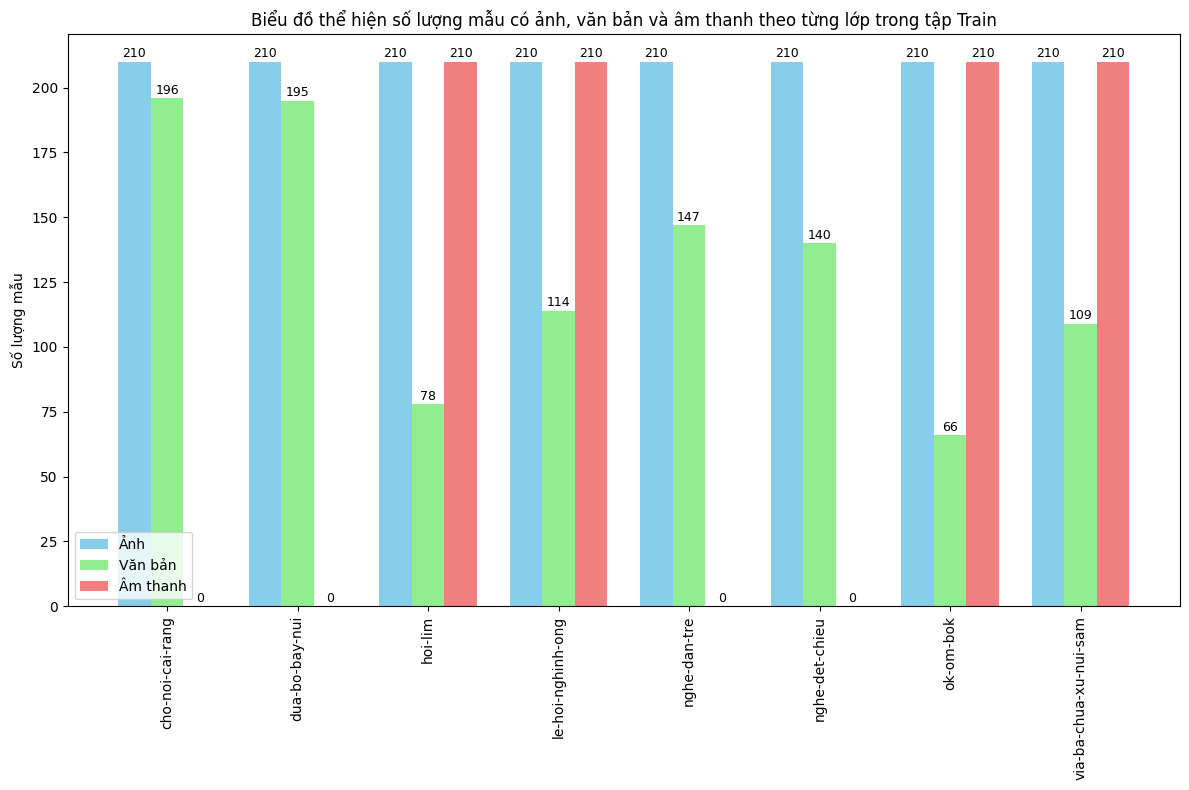
\includegraphics[width=\linewidth]{images/part-02/chap-02/sec-02/ModalNumberTrain.png}
    \caption{\centering Biểu đồ thể hiện số lượng mẫu có ảnh, văn bản và âm thanh theo từng lớp trong tập Train}
    \label{fig:ModalNumberTrain}
\end{figure}

\begin{figure}[H]
    \centering
    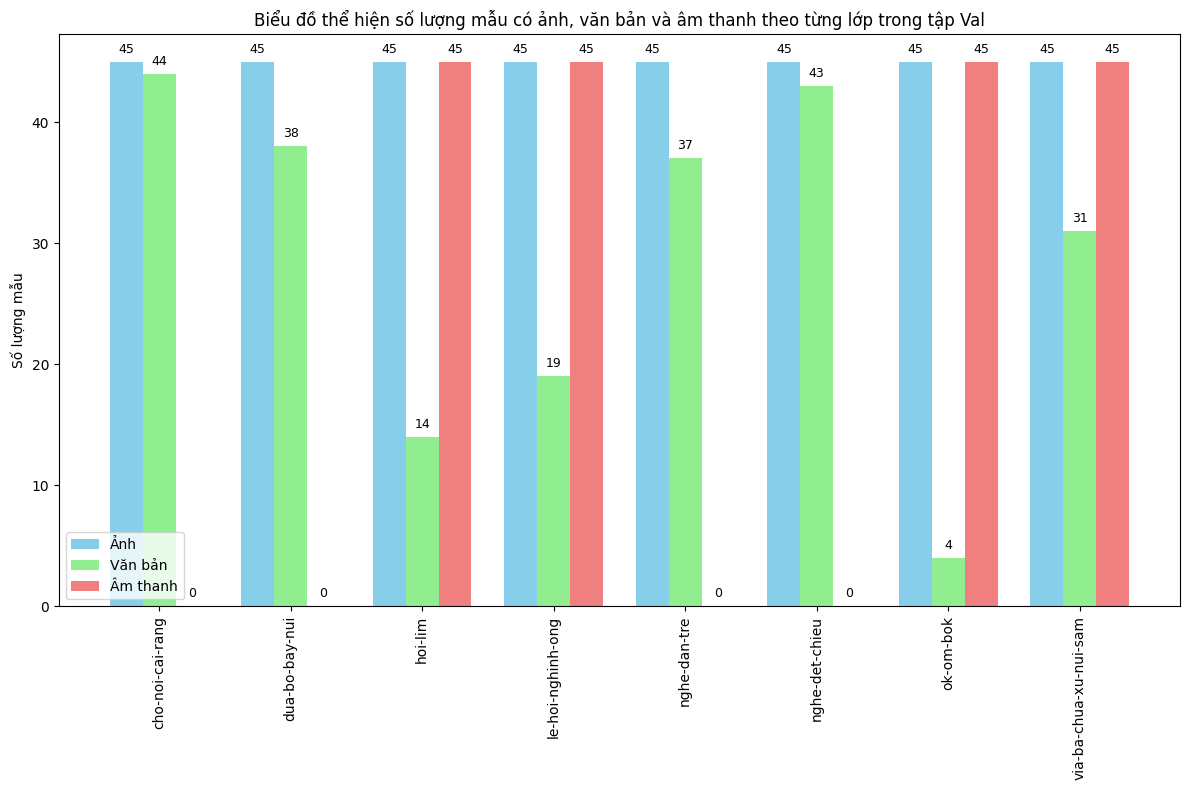
\includegraphics[width=\linewidth]{images/part-02/chap-02/sec-02/ModalNumberVal.png}
    \caption{\centering Biểu đồ thể hiện số lượng mẫu có ảnh, văn bản và âm thanh theo từng lớp trong tập Val}
    \label{fig:ModalNumberVal}
\end{figure}

\begin{figure}[H]
    \centering
    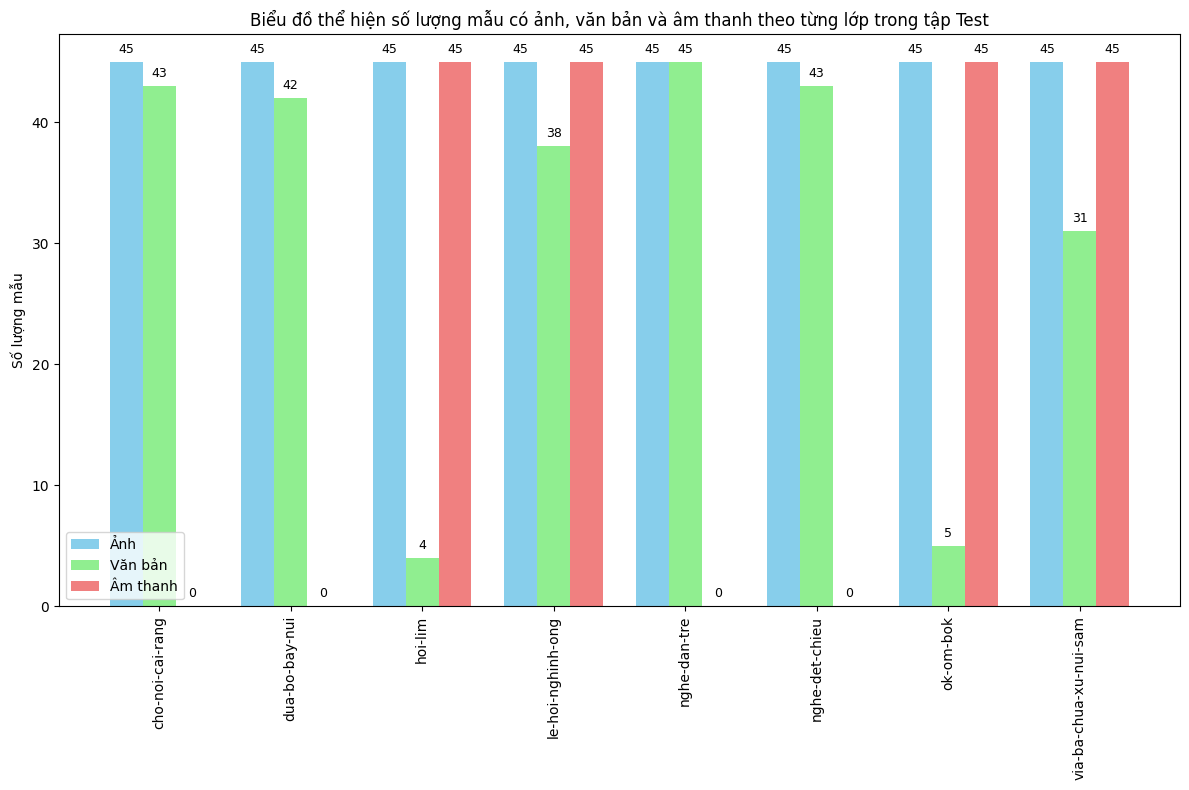
\includegraphics[width=\linewidth]{images/part-02/chap-02/sec-02/ModalNumberTest.png}
    \caption{\centering Biểu đồ thể hiện số lượng mẫu có ảnh, văn bản và âm thanh theo từng lớp trong tập Test}
    \label{fig:ModalNumberTest}
\end{figure}